\chapter{Úvod}

USB je najrozšírenejší sériový spôsob prenášania dát. Vznikol v druhej polovici 90. rokov 20. storočia kedy sa na pripojenie periférií k počítaču  používalo viacero rozličných portov (sériový a paralelný port, PS/2, ...). Na pripojenie základných zariadení ako myš alebo klávesnica slúžil napríklad port PS/2. Jeden z najznámejších sériových portov RS-232 zase mohol slúžiť na pripojenie tlačiarne. USB vzniklo za účelom nahradiť a zjednotiť tieto spôsoby pripojenia bežných periférií k počítaču. Zároveň ale ponúklo aj možnosť prenosu dát zo zariadení ako externé HDD. Z toho vylýva, že USB protokol je jeden z najkomplexnejších protokolov na komunikáciu aký existuje. Pre účel lepšieho pochopenia daného protokolu alebo v prípade implementácie vlastného zariadenia nám môžu pomôcť tvz. USB paket analyzátory. Ich zmysel je určitým spôsobom priblížiť a vyobraziť komunikáciu na danej zbernici. Cieľom tejto práce bude práve taktýto analyzátor zostrojiť.

\section{Základné pojmy}

V tejto sekcii si vysvetlíme niektoré základné pojmy ktoré budeme neskôr v~texte používať.

\subsubsection{Master/slave}
\subsubsection{Paket}
\subsubsection{URB}
\subsubsection{Analyzátor vs sniffer}
\subsubsection{USB zariadenie}
+HID
\subsubsection{Typy prenosov}
control,interrupt,isochornous,bulk (str. 20,21)
\subsubsection{USB deskriptor}

\section{Existujúce aplikácie}

Našu aplikáciu chceme hlavne zamerať na analýzu základných USB deskriptorov a komunikáciu so základnými perifériami. Konkrétne na užšiu podmnožinu HID zariadení ako sú myš, klávesnica a joystick.

Momentálne existuje niekoľko známych aplikácií ktoré slúžia na analýzu USB paketov. V tejto kapitole si ich zopár ukážeme a rozoberieme si niektoré ich funkcie a spôsob, akým analyzujú dané pakety.

Je nutné upozorniť, že väčšina dnešných analyzátorov sú platené aplikácie, prípadne majú odomknuté len základné vlastnosti s~možnosťou dokúpenia si plnej verzie. Práve preto sme nemali možnosť si pri všetkých vyskúšať ich celú funkcionalitu a na niektoré platené funkcie máme len veľmi high-level pohľad.

\subsection*{Wireshark}

Pravdepodobne najznámejšia third-party aplikácia na~analýzu sieťových paketov. Jeho funkcionalita je veľmi rozsiahla, a~vzhľadom na~to, že sa jedná o~open-source projekt, neustále rastie. Napriek tomu, že sa zameriava hlavne na sieťové pakety, podporuje spoluprácu s~rôznymi inými sniffermi. Jeden z~takýchto snifferov je \textit{USBPcap}, ktorý zachytáva USB komunikáciu. Tým pádom je Wireshark schopný analyzovať pakety aj nad~touto zbernicou. 

Teraz si postupne ukážeme niektoré funkcie Wiresharku na konkrétnom príklade (presnejšie na zachytenej komunikácii s myšou). Medzi tie úplne základné určite patrí hexdump dát nad~ktorými prebieha analýza, ktorý je vyobrazený na obrázku~\ref{obr:uvod:wireshark_hexdump}. 

\begin{figure}[!htb]
	\centering
	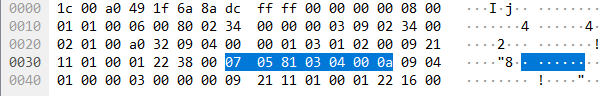
\includegraphics[width=\textwidth]{img/uvod_wireshark_hexdump}
	\caption{Ukážka hexdumpu so zvýrazneným endpoint deskriptorom.}
	\label{obr:uvod:wireshark_hexdump}
\end{figure}

Tento hexdump je tvorený dátami z jedného control prenosu, kde zariadenie posiela informácie o sebe v podobe rôznych deskriptorov. Pri pohybe myšou nad daným hexdumpom ponúka Wireshark interaktívnu odozvu, pričom farebne oddeľuje jednotlivé byty podľa ich významu. Zvýraznené byty na predchádzajúcom obrázku reprezentujú jeden endpoint deskriptor. Ďalšia užitočná vlastnosť je označenie nie len číselnej reprezentácie dát, ale takisto im odpovedajúcim tlačiteľným znakom. Tie isté dáta sa ale dajú reprezentovať viacerými spôsobmi. Môžu byť vyobrazené pomocou stromovej štruktúry, ktorá už jednotlivým bytom pridáva ich sémantický význam v slovnom tvare ako je ukázané na obrázku~\ref{obr:uvod:tree_structure} nižšie.

\begin{figure}[!htb]
	\centering
	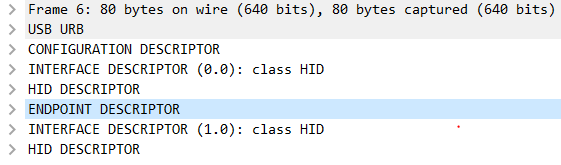
\includegraphics[width=\textwidth]{img/uvod_tree_structure}
	\caption{Ukážka reprezentácie dát pomocou stromovej štruktúry.}
	\label{obr:uvod:tree_structure}
\end{figure}

\newpage

 Jednotlivé položky si môžeme bližšie rozbaliť. Napríklad, vyššie zvýraznených 7 bytov reprezentujú endpoint deskriptor s konkrétnymi hodnotami čo ukazuje obrázok~\ref{obr:uvod:endpoint}.

\begin{figure}[!htb]
	\centering
	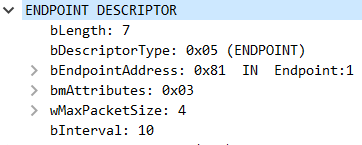
\includegraphics[width=\textwidth]{img/uvod_endpoint}
	\caption{Endpoint deskriptor reprezentovaný dátami zvýraznenými na obrázku vyššie.}
	\label{obr:uvod:endpoint}
\end{figure}

Medzi viac špecifické funkcie patrí detailnejšie vyobrazenie jednotlivých bytov a~ich význam, ako je možné vidieť nižšie na~obrázku~\ref{obr:uvod:byte_detail_foto}. Túto vlastnosť aj napriek jej využitiu mnohé konkurenčné aplikácie postrádajú.

\begin{figure}[!htb]
	\centering
	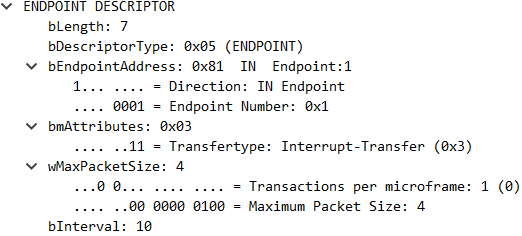
\includegraphics[width=\textwidth]{img/uvod_byte_detail}
	\caption{Ukážka vyobrazenia jednotlivých bytov.}
	\label{obr:uvod:byte_detail_foto}
\end{figure}

Jeho výhoda je hlavne v~tom, že podporuje širokú škálu deskriptorov a~plná verzia programu je dostupná úplne zadarmo. Z~pohľadu užívateľa je až prekvapivé, že aj~napriek rozsiahlosti programu je aplikácia veľmi user-friendly orientovaná a~dopĺňa ju veľmi intuitívne užívateľské rozhranie.

\subsection*{Device Monitoring Studio}

Aplikácia ponúka analýzu sieťových a~USB paketov, tak ako aj~analýzu komunikácie prebiehajúcej cez~sériový port.

Ako prvé na~aplikácii zaujme spôsob zvolenia si zariadenia s~ktorým bude sledovaná komunikácia. Je implementovaný štýlom stromovej štruktúry ako je ukázané na~obrázku~\ref{obr:uvod:treeview_foto}~nižšie, kde máme konkrétne označenú rovnakú myš s ktorou komunikáciu sme sledovali predchádzajúcim programom. 

\begin{figure}[!htb]
	\centering
	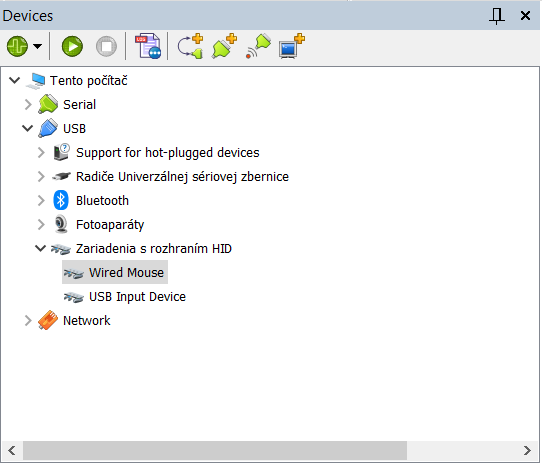
\includegraphics[width=\textwidth]{img/uvod_treeview}
	\caption{Ukážka stromovej štruktúry na~zvolenie si zariadenia s~ktorým bude zachytávaná komunikácia.}
	\label{obr:uvod:treeview_foto}
\end{figure}

\newpage

Základná verzia programu ponúka vizuálne zobrazenie \textit{URB}, tak ako aj analýzu jednotlivých paketov.
Pod analýzou si tu môžeme predstaviť ale len obyčajný hexdump ktorý neposkytuje žiadne významové oddelenie dát, tým pádom je obtiažnejšie sa v ňom zorientovať. Takisto tu nemáme žiadne sémantické vysvetlenie čo znamenajú poslané dáta (napríklad pomocou stromovej štruktúry ako to rieši konkurencia). Príklad takejto analýzy môžeme vidieť na obrázku~\ref{obr:uvod:hhd_analyza}~nižšie.

\begin{figure}[!htb]
	\centering
	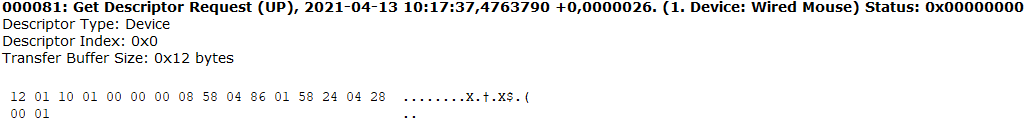
\includegraphics[width=\textwidth]{img/uvod_hhd_analyza}
	\caption{Príklad analýzy paketov.}
	\label{obr:uvod:hhd_analyza}
\end{figure}

\newpage

Vyobrazenie URB (obrázok~\ref{obr:uvod:hhd_urb}~) tak ponúka trochu obecnejší prehľad o tom, čo sa na danej zbernici deje.

\begin{figure}[!htb]
	\centering
	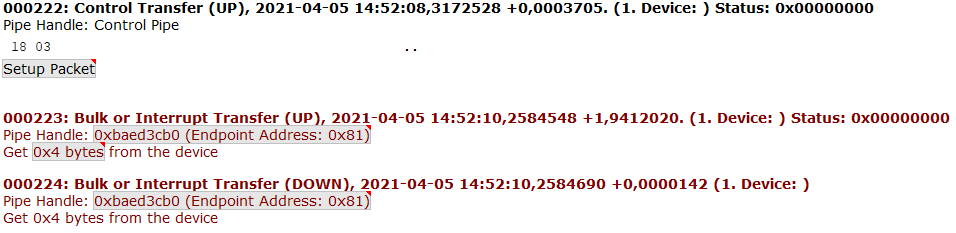
\includegraphics[width=\textwidth]{img/uvod_hhd_urb}
	\caption{Ukážka vyobrazenia URB.}
	\label{obr:uvod:hhd_urb}
\end{figure}

Pričom pri dvojkliku na šedé časti textu (napríklad \textit{Setup Packet} alebo \textit{Endpoint Address}) sa užívateľovi rozbalí okno s detailnejším popisom.
 
Zaujímavá funkcionalita ktorú ale program ponúka len v platenej verzii, je umožnenie užívateľovi priamo komunikovať so zvoleným zariadením. Môžeme mu tak posielať rôzne požiadavky (niektoré z nich sú spomenuté v USB dokumentácii v kapitole 9.4 (ODKAZ) ) ako napríklad \textit{GET\_REPORT} kde špecifikujeme \textit{Report ID} a prípadné ďalšie parametre, a zariadenie nám patrične odpovie.

Medzi zachytenými paketami sa prvotne nezobrazujú tie, ktoré označujú nakonfigurovanie daného zariadenia (je nutné ho odpojiť a~znova napojiť počas monitorovania). Užívateľské rozhranie vyobrazené nižšie pomocou obrázku~\ref{obr:uvod:hhd_interface}~,pozostáva z pomerne veľa ikoniek a celkovo sa javí ako trochu neprehľadné. Pri prvotnej interakcii s programom chvíľu trvá, kým človek nájde čo~i~len základné informácie ako napríklad hlavičky ku~jednotlivým paketom. Nepoteší ani fakt, že verzia zadarmo nedovoľuje monitorovanie dlhšie ako 10 minút a~maximálny počet monitorovaní za~jeden deň je taktiež 10.

\begin{figure}[!htb]
	\centering
	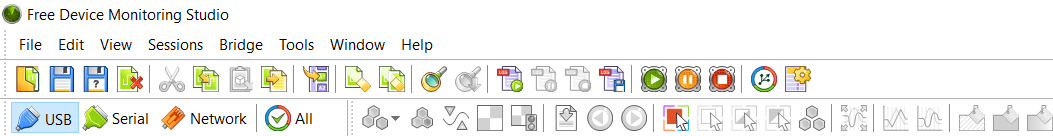
\includegraphics[width=\textwidth]{img/uvod_hhd_interface}
	\caption{Užívateľské rozhranie Device Monitoring Studio}
	\label{obr:uvod:hhd_interface}
\end{figure}

\newpage

\section{Požadované funkcie}
Na~základe minulých príkladov už existujúcich aplikácií sme si mohli všimnúť, že všetky obsahujú niekoľko základných funkcií, ktoré by mal obsahovať každý analyzátor. V~tejto sekcii zhrnieme funkcie, ktoré sme si zvolili pre našu aplikáciu. Zo~základných funkcií sme si vybrali tie, ktoré považujeme za~absolútne nevyhnutné pre každý analyzátor. Následne sme sa niekoľko z~nich pokúsili akýmsi spôsobom vylepšiť tak, aby maximalizovali ich využiteľnosť a~zároveň čo najlepšie zlepšili prácu s~aplikáciou jej užívateľovi. Zároveň ich dopĺňame o~pokročilejšie funkcie z~ktorých sú niektoré viac špecificky zamerané pre účely ktoré by sme chceli dosiahnuť v našej aplikácii.

Ako prvé by sme si mali zadefinovať platformu na ktorú budeme cieliť s našou aplikáciou:
\begin{enumerate}[label=\textbf{P\arabic*}]
	\item \label{uvod:poz:platforma} Cieľová platforma našej aplikácie by mala byť Windows. 
\end{enumerate}

Našu aplikáciu by sme chceli zamerať už na jednotlivú analýzu paketov a nie ich zachytávaniu. Z toho vyplývajú nasledujúce požiadavky:
\begin{enumerate}[label=\textbf{P\arabic*},resume]
	\item \label{uvod:poz:analyza} Mala by byť schopná analyzovať USB pakety zachytené do~súboru v~rozumnom formáte pomocou predom definovaného snifferu.
	\item \label{uvod:poz:analyza_real_time} Mala by byť schopná analýzy paketov v reálnom čase. To znamená, že bude podporovať čítanie súboru súvisle s tým ako do neho bude zapisovať iný software (za predpokladu, že to daný software povoľuje).
\end{enumerate}

Vzhľadiska zamerania našej aplikácie na základnú podmnožinu USB deskriptorov si zadefinujeme nasledujúcu požiadavku:
\begin{enumerate}[label=\textbf{P\arabic*},resume]
	\item \label{uvod:poz:deskriptory} Mala by podporovať sémantickú analýzu (vyobrazenie pomocou stromovej štruktúry) pre~všetky základné USB deskriptory spomenuté v~USB 2.0 dokumentácii(ODKAZ kapitola 9.6)~(ako napríklad \textit{Device descriptor}, \textit{Interface descriptor}, \textit{Endpoint descriptor},...).
\end{enumerate}

Požiadavky na samotnú analýzu sú:
\begin{enumerate}[label=\textbf{P\arabic*},resume]
	\item \label{uvod:poz:hexdump} Mala by vedieť rozumne zobraziť dáta ktoré daný sniffer zachytí a~uloží. Pod pojmom rozumne myslíme spôsob zobrazenia pomocou hexdumpu.
	\item \label{uvod:poz:data_highlight} Mala by uľahčiť používateľovi orientáciu v~hexdumpe. Jednotlivé znaky budú farebne označené na~základe ich významu (hlavička paketu, rôzne typy deskriptorov, ...).
	\item \label{uvod:poz:zobrazenie_paketov} Mala by na prvý pohľad jasne zobraziť základné informácie o~každom analyzovanom pakete (ako napr. dĺžka paketu, typ prenosu, ...) a~pri~bližšom skúmaní jednotlivých paketov detailnejšie zobraziť celú jeho hlavičku.
	\item \label{uvod:poz:paket_detail} Detailnejšie informácie o~pakete budú zobrazované na~základe interakcie užívateľa s~aplikáciou.
	\item \label{uvod:poz:show_bits} V~miestach kde to dáva zmysel, by aplikácia mala byť schopná zobrazovať význam dát až na~úrovni jednotlivých bitov.
\end{enumerate}

Vzhľadom na zamerianie sa na užšiu podmnožinu HID zariadení doplníme nasledujúce požiadavky:
\begin{enumerate}[label=\textbf{P\arabic*},resume]
	\item \label{uvod:poz:report_desk_parser} Mala by byť schopná rozparsovať \textit{HID Report Descriptor} takým štýlom, aby bolo neskôr možné sématnicky reprezentovať input určitých HID zariadení.
	\item \label{uvod:poz:hid_analyza} Mala by byť schopná vhodným spôsobom vizuálne zobraziť sémantický význam dát posielaných danou podmnožinou HID zariadení, do~ktorej patrí myš, klávesnica a~joystick.
\end{enumerate}

\section{Ciele práce}

Celkové ciele tejto práce sú následovné :

\begin{enumerate}[label=\textbf{C\arabic*}]
	\item \label{uvod:ciel:aplikacia} Vytvoriť funkčný analyzátor ktorý spĺňa všetky požadované funkcie~\ref{uvod:poz:platforma}\=/\ref{uvod:poz:hid_analyza}
	\item \label{uvod:ciel:rozsiritelnost} Návrh programu musí byť dostatočne obecný aby splňoval nasledujúce:
	\begin{itemize}
		\item \label{uvod:ciel:roz_USB} Jednoduché rozšírenie o~analýzu ďalších typov USB prenosov.
		\item \label{uvod:ciel:roz_HID} Jednoduché pridanie sémantickej analýzy pre~ďalšie HID zariadenia.
	\end{itemize}
\end{enumerate}